%\begin{refsection}
\section{Introduction}


Modern deep neural networks (DNNs) are complex,
and often contain millions of parameters spanning
dozens or even hundreds of layers~\cite{he2016deep,huang:2017}.
%
This complexity translates into substantial memory and runtime costs
on hardware platforms at all scales.
%
Recent work has demonstrated that DNNs are often over-provisioned and can be compressed without appreciable loss of accuracy.
Model compression can be used to
reduce both model memory footprint and inference latency using techniques such as
weight pruning~\cite{han2015learning,luo2017thinet},
quantization~\cite{gupta2015deep}, and low-rank
factorization~\cite{jaderberg2014speeding,denton2014exploiting}.
%
Unfortunately, the requirements of
different {\em compression contexts}---DNN structure,
target hardware platform, and the user's optimization objective---are often in conflict.
%
The recommended compression strategy for reducing inference latency
may be different from that required to reduce total memory footprint.
%
For example, in a Convolutional Neural Network (CNN),
reducing inference latency may require pruning filters to realize speedups on real hardware~\cite{li2016pruning}, while reducing memory footprint may be accomplished by zeroing out individual weights.
%
Similarly, even for the {\em same optimization objective},
say reducing inference latency, one may employ filter pruning for a CNN,
while pruning 2-D blocks of non-zero weights~\cite{gray:2017} for a
language modeling network such as Transformer~\cite{vaswani:2017},
since the latter has no convolutional layers.
%
Thus, it is crucial to enable convenient expression of 
alternative compression schemes, yet
none of today's model compression approaches help the designer
tailor compression schemes to their needs.


\begin{figure}[!h]
\centering
%\fbox{\rule{0pt}{2in} \rule{0.9\linewidth}{0pt}}
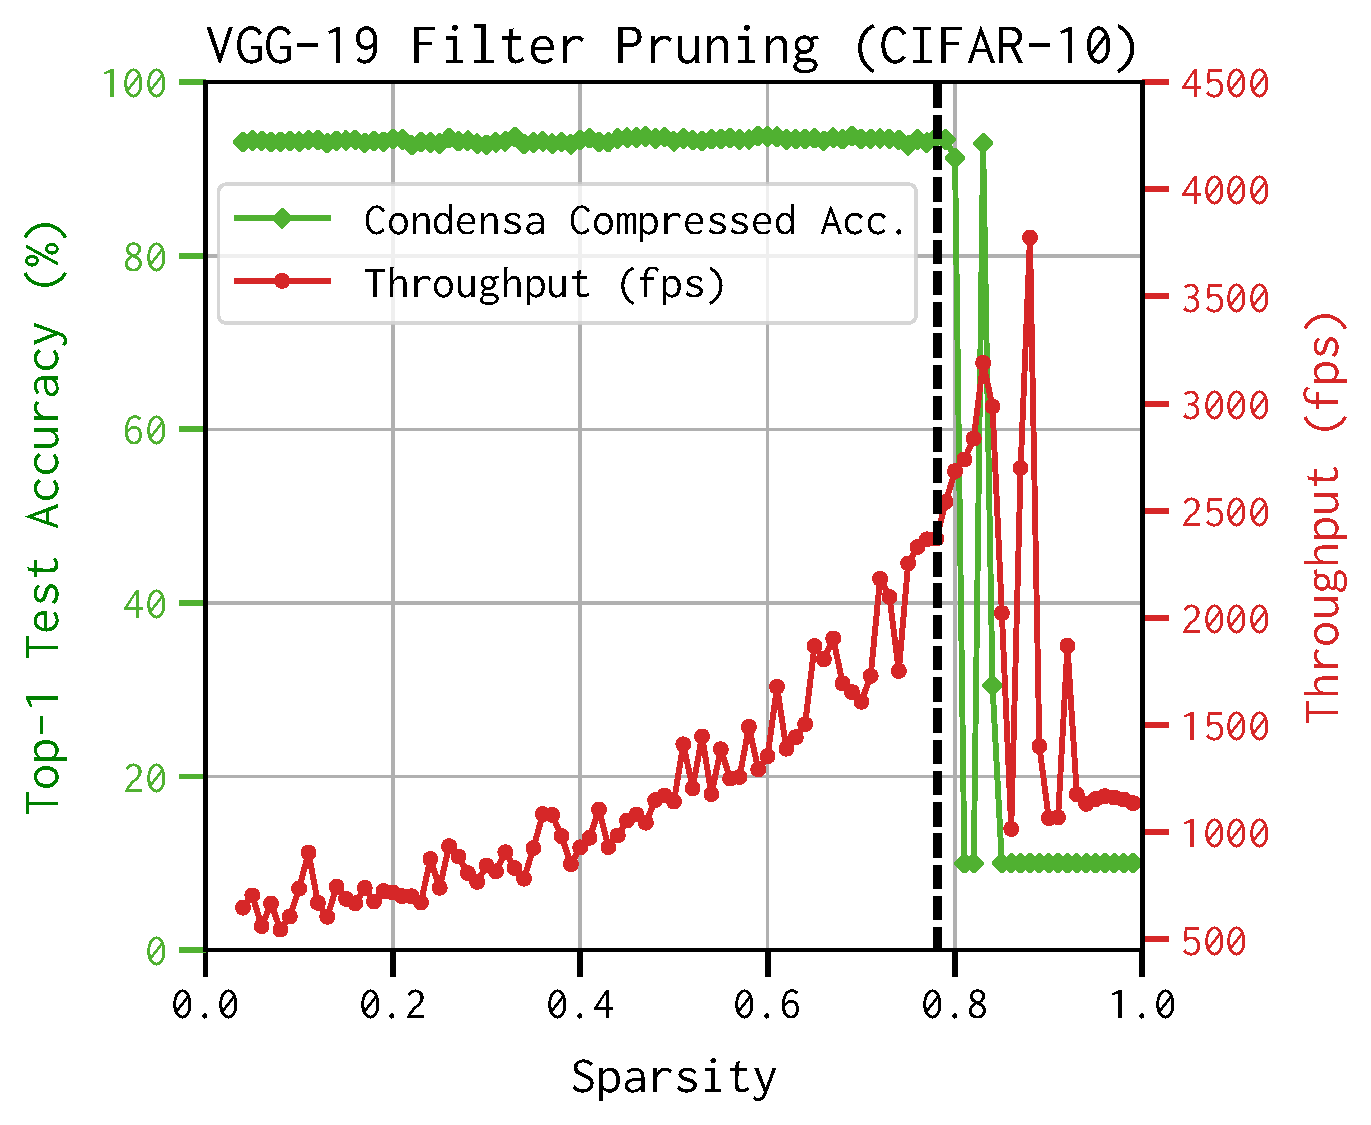
\includegraphics[width=0.5\linewidth]{img/vgg19_bn_filter_intro_v2.pdf}
%\vspace{-10pt}
\caption{Top-1 test accuracy (green) and throughput (red) vs.\ sparsity for VGG-19 on CIFAR-10.
\algoName is designed to solve constrained optimization problems of the form ``maximize throughput, with a lower bound on accuracy". In this case, \algoName automatically discovers a sparsity (vertical dashed line) and compresses the model to this sparsity,
improving throughput by $2.59\times$ and accuracy by $0.36\%$.
}
\vspace{-10pt}
\label{fig:vgg-intro}
\end{figure}

%Current approaches to model compression
%also require manual specification of compression hyperparameters, such
%as the target sparsity ratio, which is the proportion of zero-valued parameters in %the
%compressed model vs.\ the original.
%
Current approaches to model compression
also require manual specification of compression hyperparameters, such
as {\bf target sparsity}---{\em the proportion of zero-valued parameters in the
compressed model vs.\ the original.}
%
However, with current approaches, finding the best sparsity 
often becomes a trial-and-error search, with
each such trial having a huge cost (often multiple days for large models such as BERT) and involving training the compressed model to convergence,
only to find (in most cases) that the compression objectives are not met.
%
The main difficulty faced by such unguided approaches is
that sparsities 
vary unpredictably with changes in the compression context,
making it very difficult to provide users with any guidelines, whatsoever.
%
Therefore, automatic and {\em sample-efficient} approaches that minimize the number of trials are crucial
to support the needs of designers who must adapt
a variety of neural networks to a broad spectrum of platforms targeting a wide
range of tasks.

To address the above-mentioned problems of flexible expression of compression strategies, automated compression hyperparameter inference, and sample efficiency, we introduce \algoName, a new framework for programmable model compression.
\begin{figure*}[tbp]
\centering
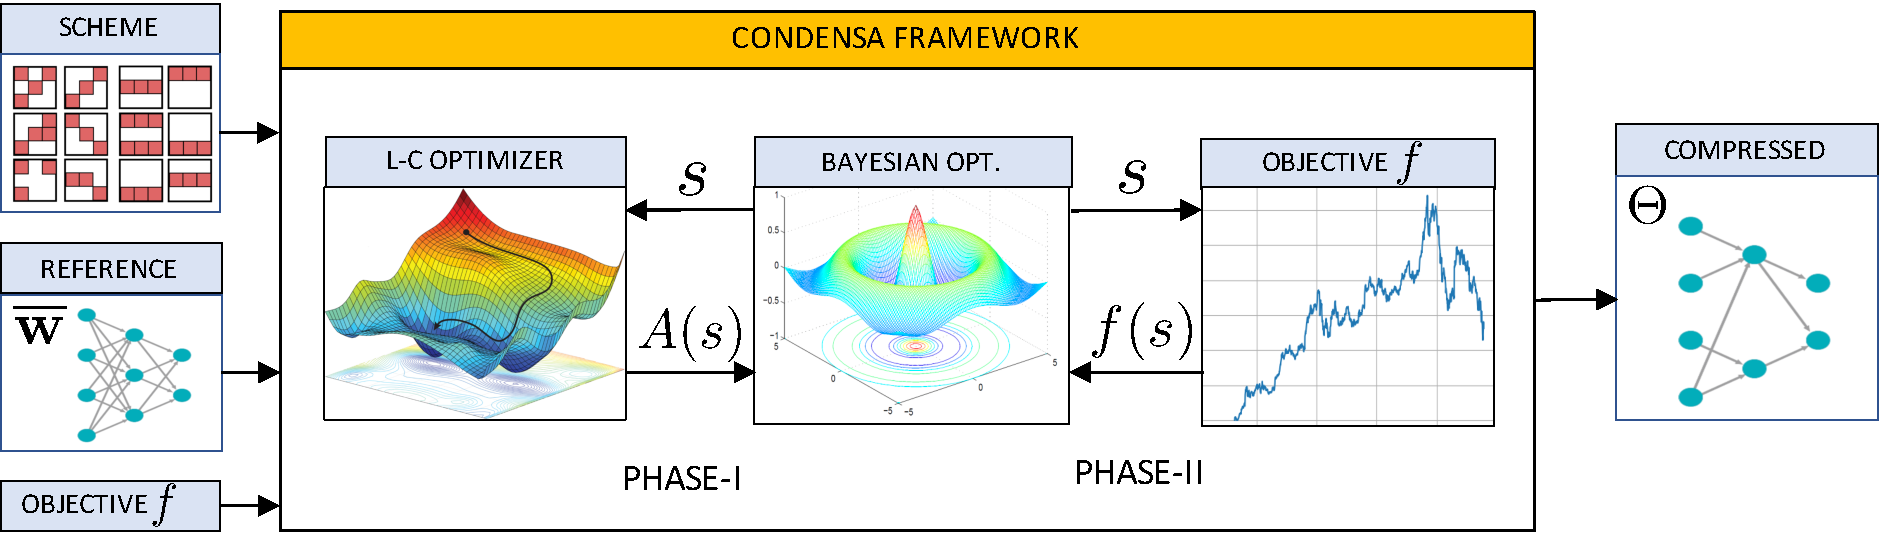
\includegraphics[width=\textwidth]{img/Overview_R4.pdf}
\caption{\algoName framework overview. The user provides the pre-trained model ($\overline{\bw}$), a compression scheme, and an objective function $f$. \algoName uses the Bayesian and L-C optimizers to infer an optimal target sparsity $s^*$ and corresponding compressed model $\Theta$.}
\label{fig:condensa}  
\end{figure*}

\begin{figure}[tb]
	\lstinputlisting[label=code:condensa,caption={Example usage of the \algoName library.}]{code/condensa.py}
\end{figure}

\begin{table}[tb]
\centering
        \begin{tabularx}{\linewidth}{ l  X }
				\hline
				\textbf{Scheme} & \textbf{Description} \\ \hline
				\texttt{Quantize(dtype)} & Quantizes network weights to given datatype \texttt{dtype}. \\ \hline
				\texttt{Prune()} & Performs unstructured pruning of network weights. \\ \hline
                \texttt{NeuronPrune(criteria)} & Aggregates and prunes neurons (1D blocks) according to \texttt{criteria}.\\ \hline
				\texttt{FilterPrune(criteria)} & Aggregates and prunes filters (3D blocks) according to \texttt{criteria}. \\ \hline
				\texttt{StructurePrune(criteria)} & Combines neuron and filter pruning.\\ \hline
				\texttt{BlockPrune(criteria, bs)} & Aggregates and prunes n-D blocks of size \texttt{bs} according to \texttt{criteria}.\\ \hline
				\texttt{Compose(slist)} & Composes together all schemes in \texttt{slist}.\\ \hline
           \end{tabularx}
	\caption{List of pre-built compression schemes in \algoName.}
	\label{tab:schemes}
\end{table}


As an illustration of the level of automation provided by \algoName,
consider the problem of improving the
inference throughput of VGG-19~\cite{simonyan2014very} on the CIFAR-10 image
classification task~\cite{krizhevsky2014cifar}.
%
Since VGG-19 is a convolutional neural network, one way to improve its
inference performance on modern hardware such as GPUs is by pruning
away individual convolutional filters~\cite{he2018progressive}.
%
Figure~\ref{fig:vgg-intro} shows the accuracy and throughput obtained
by \algoName on this task.
%
Here, we plot the compressed model's top-1 test accuracy and throughput as a function of the sparsity (green and red lines,
respectively).\footnote{Note that these curves are not known a priori and
are often extremely expensive to sample;
they are only plotted here to better place the obtained solution in context.}
%
\algoName's solution corresponds to a sparsity of $0.79$
and is depicted as the vertical dashed line.
%
This result is significant for two reasons: (1) using the \algoName library,
the filter pruning strategy employed for this experiment was expressed in
less than 10 lines of Python code, and (2) the optimal sparsity of
$0.79$ that
achieves throughput and top-1 accuracy improvements of $2.59\times$ and $0.36\%$, respectively,
was obtained automatically by \algoName using a sample-efficient constrained
Bayesian optimization algorithm.
%
Here, the user didn't have to specify any
sparsities manually, and instead only had to define a domain-specific
objective function to maximize (inference throughput, in this case).

%%%%%%%%%%%%%%%%%%%%%%%%%%%%%%%%%%%%%%%%%%%%%%%%%%%%%%%%%%%%%%%%%%%%%%%%%%%%%%%%%%%%%%%%%
%%%%% CIE
%%%%%%%%%%%%%%%%%%%%%%%%%%%%%%%%%%%%%%%%%%%%%%%%%%%%%%%%%%%%%%%%%%%%%%%%%%%%%%%%%%%%%%%%%

 Now, an increasing number of applications, including autonomous driving~\cite{teslacrash17}, surveillance~\cite{yang2018low}, and voice assistance systems~\cite{alam2020survey}, demand ML models that can be deployed on low-power and low-resource devices, and typically have strong latency requirements \cite{dennis2020edgeml, kusupati2018fastgrnn}. In such applications, the notion of {\em model compression} has gained popularity; at a high level, model compression involves taking a {\em reference model} and producing a {\em compressed model} that is lightweight in terms of computational requirements, while being functionally equivalent to the reference model (i.e., produces the same classification outputs on all inputs).
Model compression has been studied extensively in computer vision as well as other domains~\cite{cheng2017survey}, leveraging techniques such as 
structured 
weight pruning~\cite{wang2019structured,mccarley2020structured,frankle2018lottery, luo2017thinet,dong2017more,molchanov2016pruning}, quantization~\cite{zhu2016trained, gong2014compressing} and 
low-rank factorization~\cite{kossaifi2020factorized,lebedev2014speeding, , , }. 
% These individual compression schemes as well as their combinations can be expressed together in programmable compression systems such as~\cite{joseph2019condensa}. %and these individual compression
% %schemes for pruning and quantization and their interesting combinations can be expressed in \algoName and all these schemes are but some of the methods used for this task. 
% \sscmt{This violates double-blind and makes it evident that the authors are the same. I would suggest to not mention the name Condensa at all since we never used it explicitly for the final experiments.}
%
Many of these methods rely on making structural modifications to the network and then fine-tuning to potentially regain some of the accuracy loss.

However, in spite of its power and potential, model compression techniques are known to have drawbacks~\cite{8711062}. For example, certain classes may be unfairly affected in terms of classification accuracy compared to others; this may lead to unfair outcomes, e.g., ethnicity-based discrimination in facial~\cite{chekanov2017evaluating} or speech recognition~\cite{buolamwini2018gender}.
%
Mitigating this impact of compression is particularly
urgent, given the widespread use of compressed deep 
neural networks in resource-constrained and sensitive 
domains such as 
%
%
%
health care diagnostics~\cite{xie2019automated, %(Xie et al., 2019; 
gruetzemacher20183d,    %Gruetzemacher et al., 2018; 
badgeley2019deep,       %$Badgeley et al., 2019;
oakden2020hidden},       %Oakden-Rayner et al., 2019),
%
%
self-driving cars~\cite{teslacrash17}, %(NHTSA, 2017)
%
facial recognition software~\cite{
buolamwini2018gender% Buolamwini
 % Gebru, 2018b). 
}, and
%
human-resource management~\cite{amazon18, 
yourface19}. % Harwell2019
%
%
For these tasks, the trade-offs incurred by 
compression will be intolerable given the huge impact 
on human welfare.

Another class of drawbacks come from complex inputs~\cite{kendall2017uncertainties,wilmanski2016complex}, e.g., in an image with different components, the reference model may `focus' on certain aspects/features while the compressed one may focus on others. 
These drawbacks may be attributed to the fact that network compression is usually performed with the goal of simply matching the overall accuracy of the reference model. This leads us to the following question: {\em can  compression schemes ensure that the compressed and reference networks are close at a semantic or feature level?}
This question is challenging because networks can have different number of layers, features per layer and different connectivity structures. Moreover, the answer generally depends on the architecture of the reference network and the task at hand. The goal of our paper is to use ideas from knowledge distillation (such as logit pairing~\cite{ba2014do, hinton2015distilling}) to introduce new terms into the objective function of a compression scheme and help answer the above question. With new loss terms, the challenge now is to understand the relative importance of the terms and measure the impact they have on the overall objective.
%how to measure the impact of adding new terms into the objective. 

\paragraph{Compression Impacted Exemplars (CIEs)} To measure the impact of compression, we use a metric proposed in a series of work by Hooker et al.~\cite{hooker2020characterising}: counting the number of classification mismatches between the reference and the compressed model.\footnote{\label{footnote:cie-cie}Note that~\cite{hooker2020characterising} used the slightly different name of Compression {\em Identified} Exemplars; our modification is done to ensure compatibility with a similar notation for segmentation that we will define later.} This number can be {\em more informative than purely the accuracy} of the compressed model. For example, a lot of research has focused on making models more unbiased, more fair and more robust. If we have a reference model obtained using such methods, we would wish to have compression methods to preserve these properties. In fact, we consider a subset of CIEs (which we call \textit{CIE-Us} and report both CIE and \textit{CIE-U} numbers.

\begin{figure*}[!t]
\centering
  % \includegraphics[width=0.8\textwidth,height=10cm]{CVPR2021/img/FinalIntroFigure.pdf}
  \includegraphics[width=\textwidth]{img/FinalIntroFigure.pdf}
  \caption{Overview of our CIE reduction framework using label preservation-aware loss functions.}
  \label{fig:overview}
\end{figure*}

%\end{refsection}